\section{Instrument Design}
\label{IPR_design}
This section is related to the instrument concept, design and its characteristics 
\subsection{Instrument Concept}
\ac{IPR} is an active radar sounding instrument which is based on the transmission of the electromagnetic waves at low frequency and uses reflected echoes from the surface and subsurface to image the subsurface structure that contains the information about the interfaces of different subsurface layers. Thanks to the relatively low frequency and the nadir-looking geometry, only a portion of the transmitted pulse is backscattered from the surface, while a significant part of the pulse is propagated to the subsurface icy layers \cite{Gany_SRS}. The coherent echoes backscattered from the subsurface interfaces within each resolution cell (defined by the along-track and across-track resolutions) are detected by the receiver and visualized in the resulting radargram \cite{Gany_SRS}. Working principle of the \ac{IPR} for \ac{JGO} is shown in figure \ref{fig:IPR_concept}. Off-nadir echo (e.g from point B in figure \ref{fig:IPR_concept}) will reach the antenna at the same time as the subsurface echo thus masking it. So clutter estimation and rejection is done in signal processing for both along track and across track direction.\\
%
The \ac{IPR} for the \ac{JGO} system is based on a mature and experienced technology that has flight heritage for two different Mars Missions (MARS Express, with the \ac{MARSIS} instrument; NASA Reconnaissance Orbiter with \ac{SHARAD} with slight variations to full fill  the mission objectives of the \ac{JGO}.
%
\begin{figure}[bht]
\centering
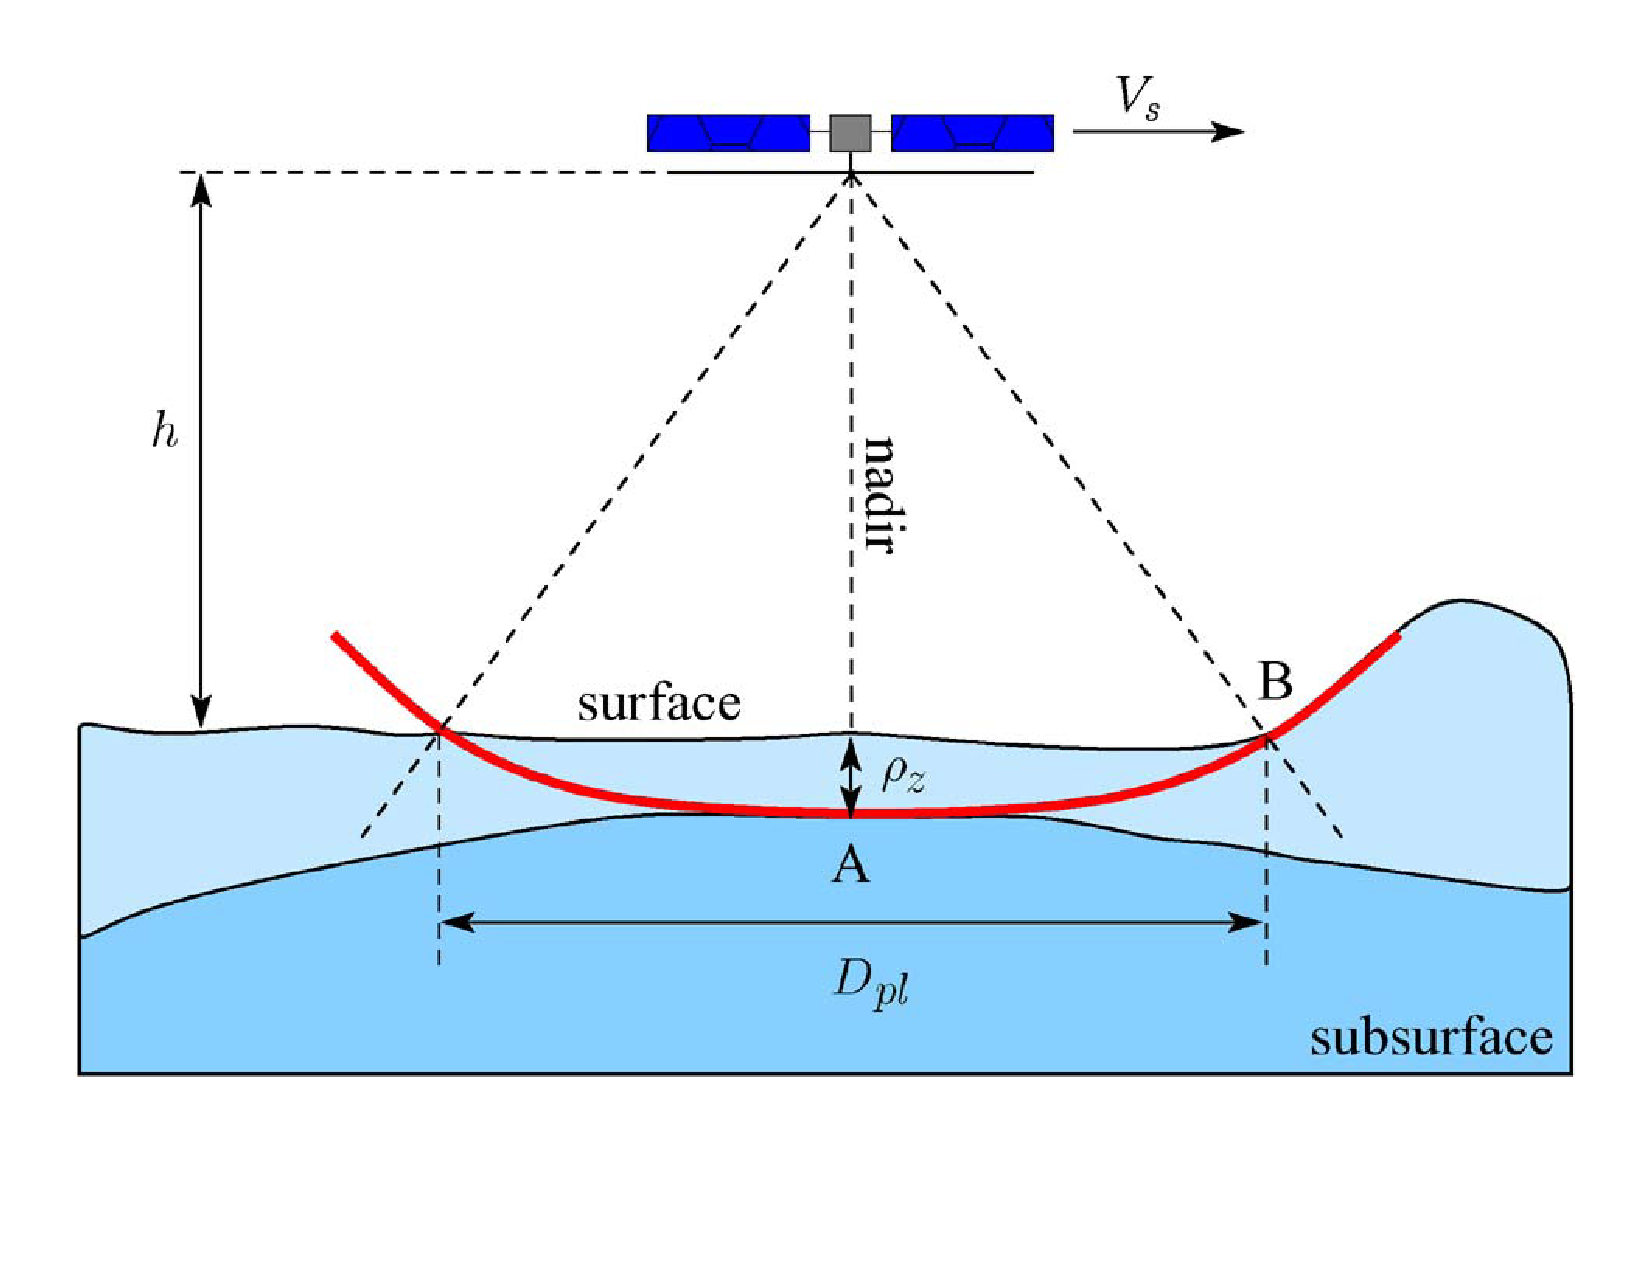
\includegraphics[scale=0.5]{Figures/IPR_Concept.pdf}
\caption{Geometry of \ac{IPR} sounder instrument \cite{Gany_SRS}} 
\label{fig:IPR_concept}
\end{figure}
%
\subsection{Instrument Description}
Architecture of the \ac{IPR} is shown in figure \ref{fig:IPR_achitecture} which is mostly inherited from the SHARAD instrument. It  consists of four main subsystems; \ac{DES}, \ac{TFE}, \ac{RX} and dipole antenna.
\subsubsection{Digital Electronics}
\ac{DES} is responsible for the radar signal generation. In the design of \ac{IPR}, concept of software defined radar is utilized with maximum processing in software domain while minimizing the analog electronics. So in order to maintain the high fidelity of the signal, frequency-modulated radar pulses (chirp) are digitally generated directly at the transmit frequency so that no up conversion is needed in the analog domain. Chirp modulated signal will improve the range resolution giving a gain provided by equation \ref{eq:chirp gain} even with low peak power pulses due to hardware constraints.\\
\ac{DES} is also responsible for all the command and control functions with the spacecraft bus. This controls all the timing sequences of the instrument which are derived from the master oscillator. Instrument will be interfaced to the spacecraft through \ac{DES} to receive telecommands and for sending telemetries. \ac{DES} provides the processing capabilities to raw data collected during observation and packetizes them into science data packet together with the auxiliary information for ground processing.
\begin{equation}
\eta_{z} = \tau B_{w}
\label{eq:chirp gain}
\end{equation}
%
\subsubsection{Transmitter}
In the \ac{TFE} section, Frequency modulated chirp signal is first amplified to the desired power level and then though the duplexer it goes to the matching network. Duplexer isolates the transmitter from receiver while permitting the use of same antenna. Matching network maximizes the radiated power.
%
\subsubsection{Receiver}
The received signal is first amplified with low noise amplifier and then filtered to reduce the noise in the receiver bandwidth. The amplified signal is converted into digital domain using \ac{ADC} and routed to the \ac{DES} where it is down converted and down sampled.
\subsubsection{Antenna}
The antenna for \ac{IPR} is a 3.6m fold able dipole antenna developed by the North Grumrupmam called foldable flatten able tube(FFT). This technology  has been previously used for \ac{MARSIS} mission. Dipole antenna has a radiation pattern of doughnut shape with the null at the  current feed point.
\begin{figure}[bht]
\centering
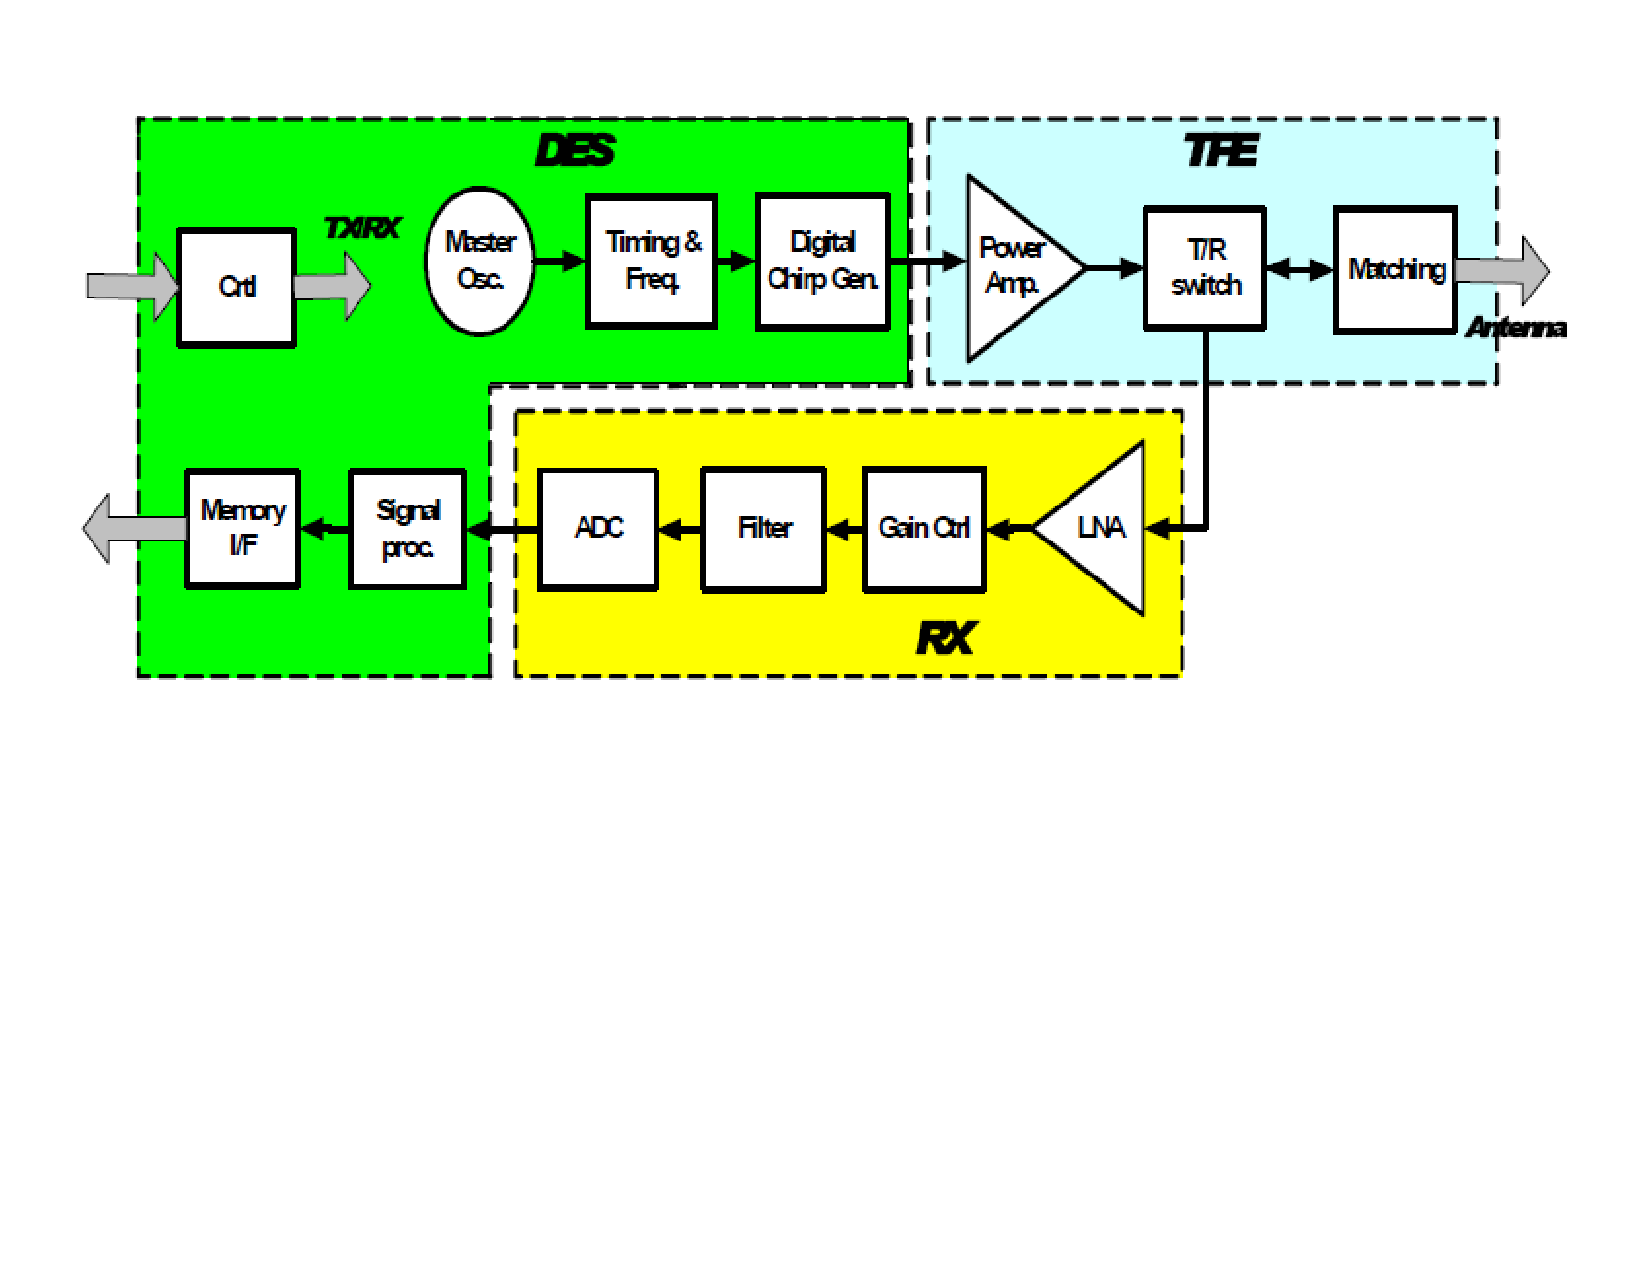
\includegraphics[scale=0.5]{Figures/IPR_Architecture.pdf}
\caption{Architecture of \ac{IPR} instrument \cite{IPR_performance}}
\label{fig:IPR_achitecture}
\end{figure}
%
\subsection{Instrument Characteristics}
The characteristics and parametrs of the \ac{IPR} are listed in table which are explained in the following subsections.\\
\begin{tabular}{|c|c|}
\hline 	\textbf{Parameter}		&  \textbf{Value}\\ 
\hline  Orbit Altitude			&  $200 Km$	\\ 
\hline  Centre Frequency		&  $45 MHz$		\\ 
\hline  Chirp Bandwidth			&  $10 MHz$		\\
\hline  PRF						&  $963.39 Hz$	\\  
\hline  Pulse Width				&  $85 us$		\\ 
\hline  Ice Range Resolution	&  $8.6 m$		\\
\hline  Along Track Resolution	&  $817 m$		\\ 
\hline  Across Track Resolution	&  $4899 m$		\\ 
\hline  SNR						&  $14.7 dB$	\\ 
\hline  Power					&  $20 W$		\\ 
\hline  Mass					&  $10 Kg$		\\ 
\hline 
\end{tabular} 
\subsubsection{Central Frequency and Bandwidth}
Radar frequency determines the penetration capability of the radar, while bandwidth of the transmitted pulse determines range resolution \cite{penetrartion}. From the Jovian radiation spectrum, it is clear that the frequency cutoff for the Jovian radio
emission affecting the subsurface radar is around 40 MHz. So, we choose 45 MHz as central frequency for the \ac{IPR} with 10 MHz bandwidth (40-50 MHz). This gives 3.6m length for the dipole antenna. Assuming pure ice ($\epsilon_{r} = 3.2$), Vertical resolution of the \ac{IPR} is 8.4 m which is calculated from equation \ref{eq:range_resolution}.
%
\begin{equation}
\rho_{z} = \dfrac{c}{2B_{w}\sqrt{\epsilon_{r}}}
\label{eq:range_resolution}
\end{equation}
%
\subsubsection{pulse repetition frequency and pulse width}
Pulse width for the \ac{IPR} is $85 us $ and \ac{PRI} is $1038 us$; giving a duty cycle of $8.2\% $. This results in \ac{PRF} of $963.39 Hz$. All these timings are shown in figure \ref{fig:PRI}. Receiving window of $165 us$ is dedicated to receive the radar echoes. Size of the receiving window is calculated by adding two way travel time in ice for $5 Km $ depth ($60 us$), chirp signal duration ($85 us$) and  a safety margin of $10 us$ on each sides. Speed of the electromagnetic wave is reduced by a factor of $1.7$ in ice. Switching time of $177 us$ from transmission to reception mode is incorporated as utilized in \ac{SHARAD} design \cite{SHARAD}.
%
\begin{figure}[bht]
\centering
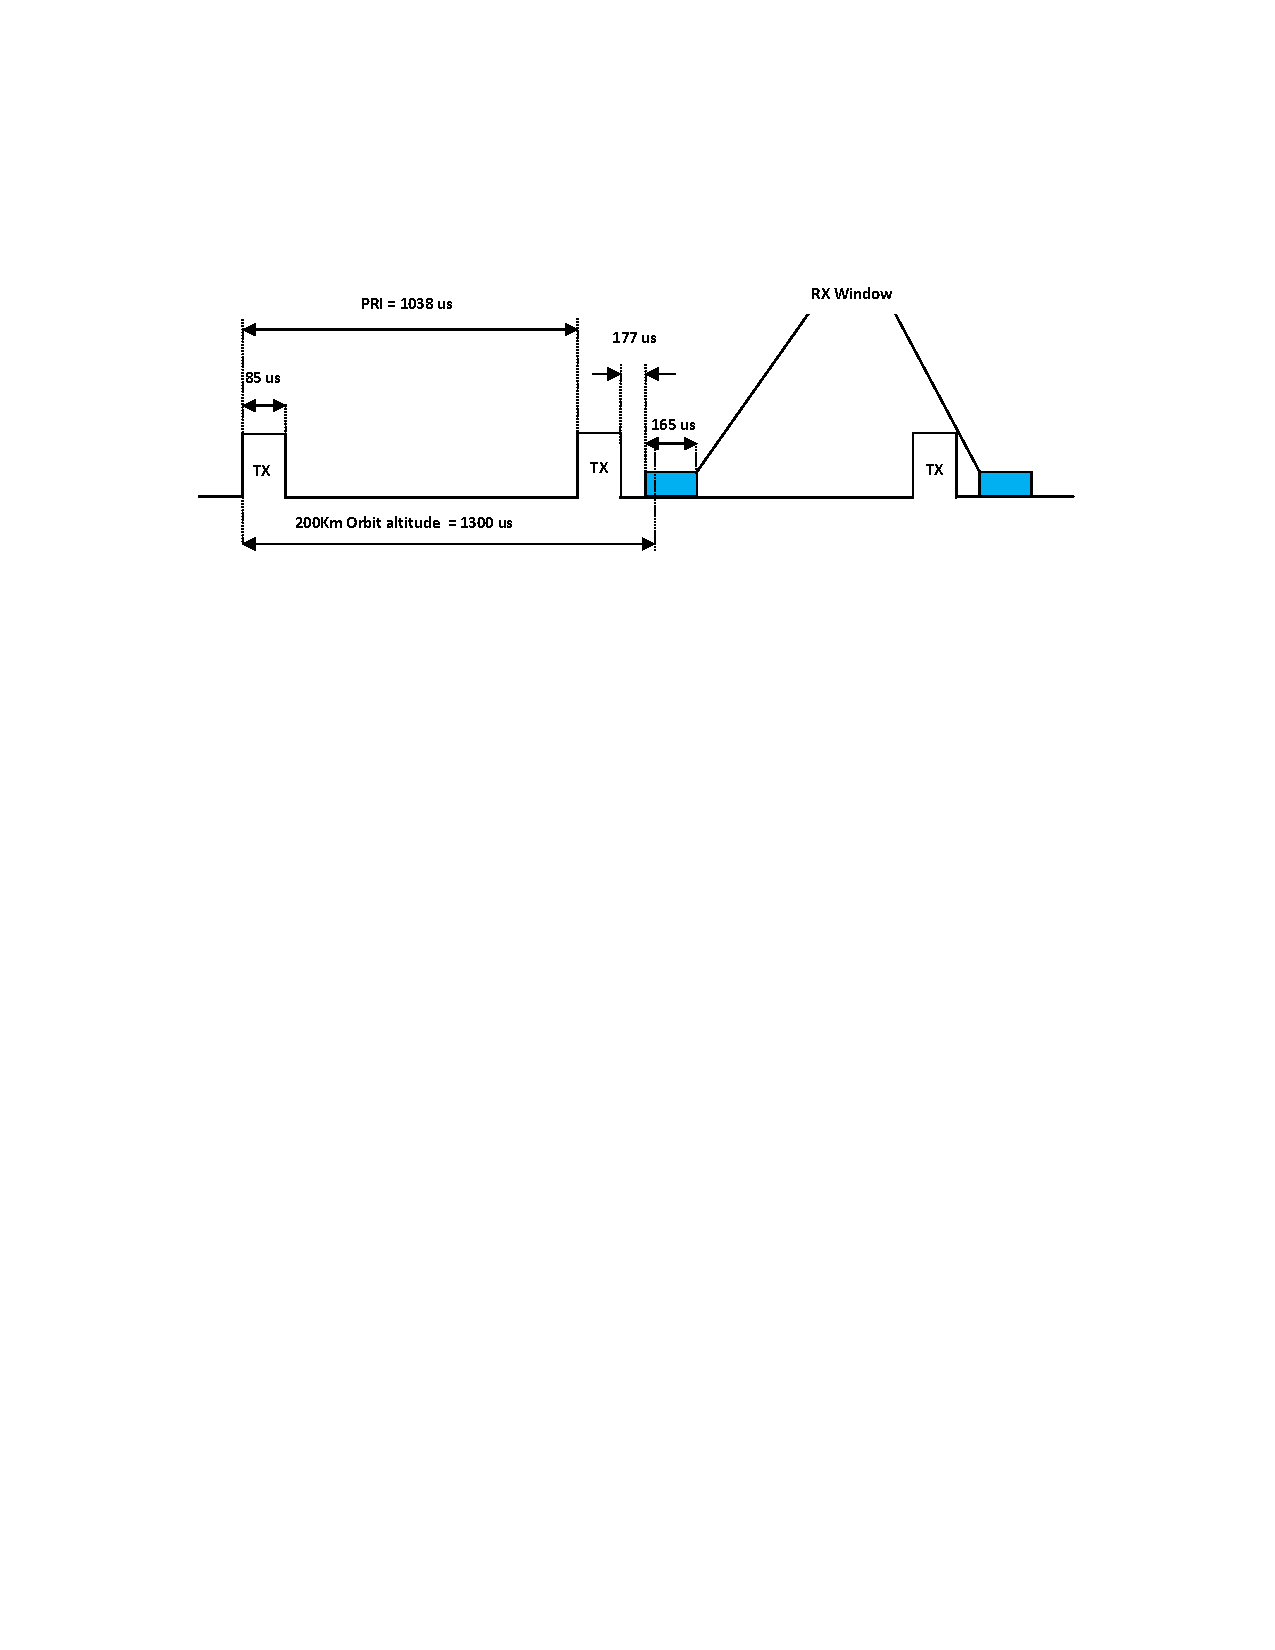
\includegraphics[scale=0.7]{Figures/PRI.pdf}
\caption{Timing diagram of Ganymede \ac{IPR}} 
\label{fig:PRI}
\end{figure}
%

\subsubsection{Signal-to-Noise Ratio}

The power of the received echo is estimated from the classical radar equation. Using the \ac{IPR} design parameters from the table, the expected level of the received power is calculated. in fact, signal level after processing is quite high as compared to received signal $P_{r}$. This is because we have two processing gain; one chirp processing gain of $29.3 dB$ given by equation \ref{eq:chirp gain} and second synthetic aperture processing gain of $28 dB$ given by equation \ref{eq:Number_pulses}. After incorporating the processing gain, signal power is given by equation \ref{eq:signal_strength} which is about $-91.7 dB$.

\begin{equation}
P_{r} = \dfrac{P_{t}\lambda^{2}\pi(\frac{D_{pl}}{2})^{2}\sigma_{o}}{4\pi^{3}h^{4}} 
	  = -139 dB + 10 log \sigma_{o}
\end{equation}
where $P_{t}$ is the transmitted power,$\lambda$ is the wavelength  and $\sigma_{o}$ is the reflection coefficient of the target surface and is statistical quantity which depends upon the dielectric properties of the two mediums at the interface and is approximated by the Kirkhhoff Approximation  and for air/ice interface it is equal to $-10dB$ \cite{MIMOSA}.
\begin{equation}
S = P_{r} + 28 +29.3
  = -81.7 dB + 10 log \sigma_{o}
\label{eq:signal_strength}
\end{equation}

Loss tangent from which the dielectric absorption is calculated depends upon the electromagnetic wave frequency and the temperature of the ice \cite{MIMOSA}. Assuming Ganymede surface temperature of 120 K and a slow linear increasing with depth of about 10 K within the first 5-km depth, \cite{Gany_SRS} calculated the attenuation of the radar signal for 20 MHz and 50 MHz. Interpolating the result for 45 MHz frequency, the attenuation is $1.2 dB per Km$ giving $12 dB$ loss for two way traversing of radar signal in 5 Km depth. So after travelling two way $5 Km $ distance signal will be $103.7 dB$.

Radar sensitivity is limited by the noise sources such present in the measurement chain. These sources include Jovian emission, galactic noise and thermal noise of the receiver.  As the central frequency and the associated bandwidth of $10 MHz$ is away from the noisy Jovian spectrum so Jovian noise is not critical. Galactic noise temperature at $45 MHz$ is about $10^{4}K$ while the thermal temperature of the radar receiver will be about  $300 K$. So, we can ignore thermal noise of the receiver and the performance of the\ac{IPR} is only limited by the galactic noise which is calculated from equation \ref{eq:galactic_noise} and is equal to $-118.6 dB$. So signal to noise ratio will be $14.9 dB$ ($\frac{S}{N_{g}}$).
\begin{equation}
N_{g} = K_{B}T_{g}B_{w}
\label{eq:galactic_noise}
\end{equation}
\\


\subsubsection{Clutter Rejection and Synthetic Aperture Processing}
As the directivity of the dipole antenna is quite low which will illuminate a large surface area of the target. This will result in echoes coming from the off-nadir along with nadir direction as shown in figure \ref{fig:IPR_concept}. This off-nadir echoes called clutter can be divided into two parts; along the track clutter and across the track clutter.\\
%
Along the track clutter will be removed by the synthetic aperture processing technique which uses the relative motion between the spacecraft and target to synthesize a large aperture which is equal to the space covered during the integration time. As \ac{IPR} is a coherent radar, it measures and records the phase history of the received signals. In order to reduce on board computation and data rate, Doppler processing is chosen unfocussed. Moreover following the \ac{MARSIS} approach \cite{MARSIS} (i.e., requiring that the signal phase variation during a synthetic aperture is smaller than $\pi/4$, the phase compensation of the echoes during the formation of a synthetic aperture is simpler and can be performed on board in real time, as only a linear phase compensation of the echoes is required \cite{Gany_SRS}.\\
%
To ensure that only coherently resolved echoes from a contiguous Fresnel zone are being illuminated, the maximum along track integration distance (the aperture; L) is the same length as the Fresnel zone.
\\
Across the track clutter is limited by the antenna pattern and will be removed by developing a simulator of the radar using a model of the overflown surface (accurately modelled at the scale of interest), which predicts the presence of clutter echoes. In this way, the corresponding echoes appearing in the measured radar-gram can be properly interpreted as clutter and then neglected \cite{SHARAD}. Some information for Ganymede was obtained through a \ac{DEM} produced from Voyager images. However, more work is necessary for deriving \acp{DEM} of different portions of Ganymede for a better understanding of the clutter issue \cite{Gany_SRS}.
As the instrument package of the \ac{JGO} mission includes radar altimeter so after modelling the Ganeymede surface, across the track clutter will be removed.

\subsubsection{Ground Resolution}
Along the track resolution:
For the unfocussed Doppler processing, along track resolution calculated using equation \ref{eq:along_track_resolution} is $817 m$. Effective integration time for unfocussed Doppler processing calculated by equation \ref{eq:integration_time} is $860 ms$ and finally the number of pulses used to make synthetic aperture is calculated by equation \ref{eq:Number_pulses} from \cite{Gany_SRS}  which comes out to 666 giving a processing gain of $28 dB$ 
%
\begin{equation}
L_{s} = \sqrt{\dfrac{h\lambda}{2}}
\label{eq:along_track_resolution}
\end{equation}
%
\begin{equation}
T_{i,eff} = \dfrac{D_{f}}{V_{s}}
\label{eq:integration_time}
\end{equation}
\begin{equation}
N = T_{i,eff}PRF 
\label{eq:Number_pulses}
\end{equation}
Across track resolution: The lateral resolution of the system is determined by the nature of the target.
Over specular surfaces (at the length scale of wavelength), where coherent reflection can be assumed, the resolution becomes that of the ``Fresnel circle'' which is 1633 m calculated using equation \ref{eq:fresenel_circle} from \cite{SHARAD}.
\begin{equation}
D_{f} = \sqrt{2h\lambda}
\label{eq:fresenel_circle}
\end{equation}
where $h$ is height and $D_{f}$ is Fresnel circle diameter.

Over rough surfaces, where incoherent scattering is assumed, the ground resolution is approximated with the first pulse limited resolution cell $D_{pl}$ as shown in figure \ref{fig:IPR_concept} . The first pulse-limited cell is represented by a circle on the ground centered in the nadir point, which diameter is given by the intersection of the wavefront with the ground surface when the transmitted wave has penetrated into the ground to a depth equal to $\rho_{z}$ \cite{Gany_SRS}. So worst case resolution for incoherent scattering calculated from equation \ref{eq:pulse_limited_cell} is 4899 m 
\begin{equation}
D_{pl} = 2\sqrt{\dfrac{hc}{B_{w}}}
\label{eq:pulse_limited_cell}
\end{equation}